\section{Super-Kamiokande and Atmospheric Neutrinos}
Interactions of cosmic rays in the upper atmosphere also produce copius neutrinos that may be used in neutrino experiments.
The hadronic shower produces pions and kaons which, in turn, decay to produce neutrinos 

\begin{equation}
\pi^+ \rightarrow \mu^+ \nu_\mu \rightarrow e^+ \nu_e \bar{\nu_\mu} \nu_\mu
\end{equation}

from the pions and from the kaons

\begin{equation}
K^+ \rightarrow \pi^+ \nu_\mu \rightarrow  e^+ \nu_e \bar{\nu_\mu} \nu_\mu \nu_\mu
\end{equation}

The neutrino flux depends on a number of parameters, including the Earth's magnetic field and temperature profile, the cosmic ray flux, and the details of hadronic interactions in air showers \cite{Honda-2015}.
The calculation of the neutrino flux predictions requires significant, dedicated simulation work, producing fluxes as both a function of energy (Figure~\ref{fig:honda_en}) and direction (Figure~\ref{fig:honda_coszen}).

\begin{figure}[!h]
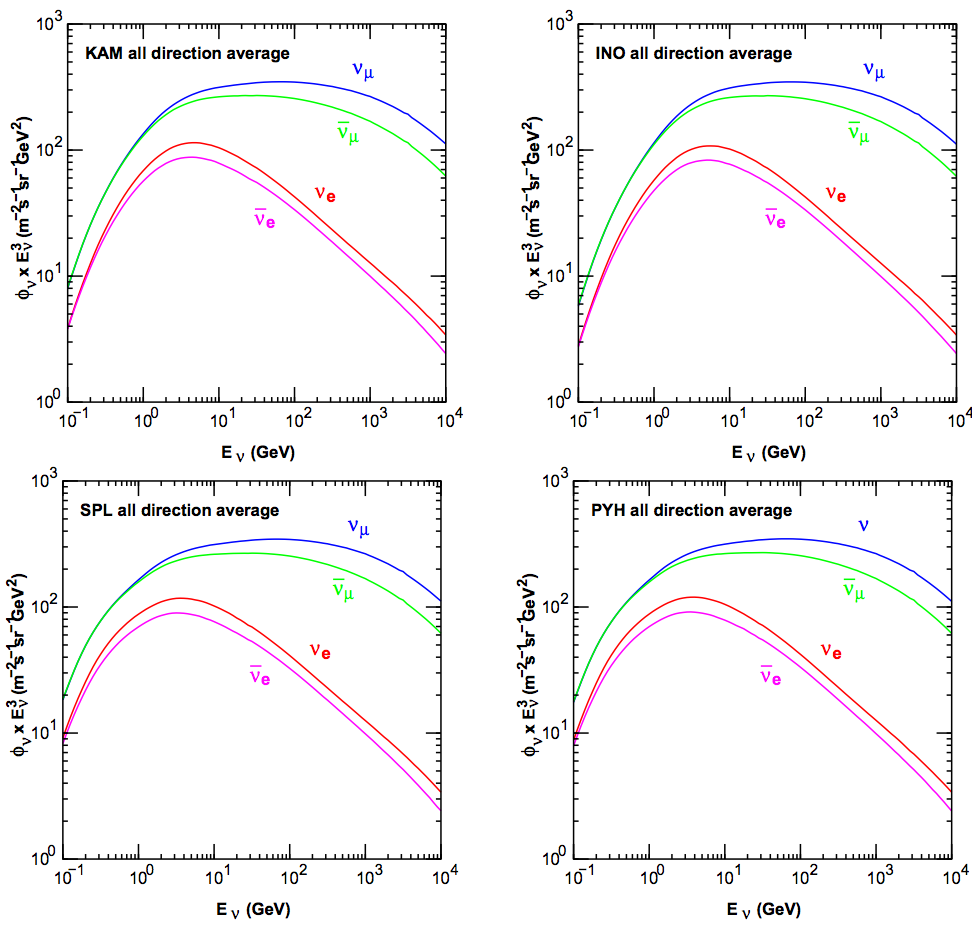
\includegraphics[width=\linewidth]{honda15_en.png}
\caption{The expected neutrino flux at Kamioka mine, Japan (Super-Kamiokande, top left), Ino Peak, India (India-based Neutrino Observator, top right), the South Pole (IceCube, bottom left), and Pyhasalmi mine, Finland (EMMA experiment, bottom right) as a function of energy. Note that the neutrino and anti-neutrino fluxes are characterized separately. The differences in the flux at each site is due to differences in the Earth's magnetic field and temperature profile. Figure taken from \cite{Honda-2015}.}
\label{fig:honda_en}
\end{figure}

\begin{figure}[!h]
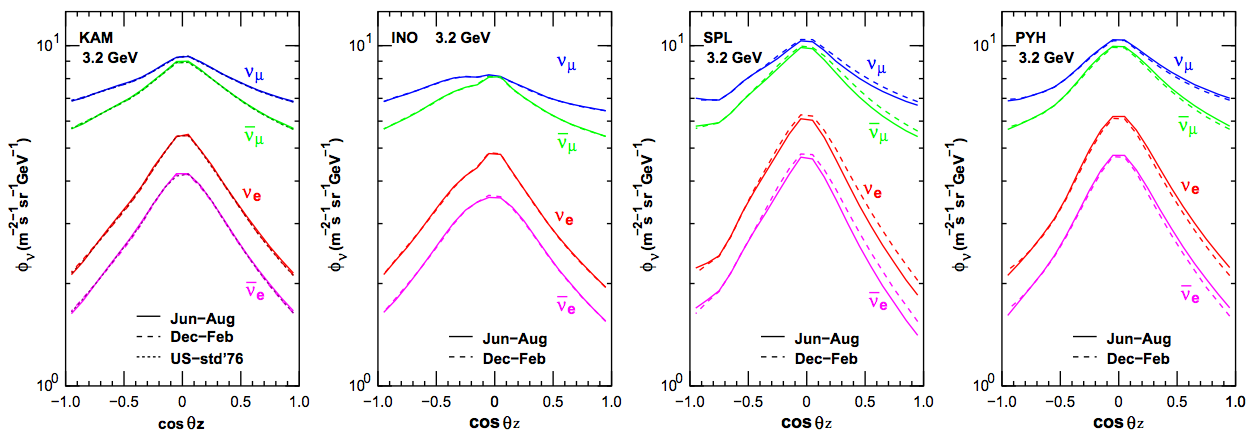
\includegraphics[width=\linewidth]{honda15_coszen.png}
\caption{The expected flux of 3.2 GeV neutrinos at Kamioka mine, Japan; Ino Peak, India; the South Pole; and Pyhasalmi mine, Finland as a function of zenith angle. A value of $\cos \theta_Z=-1$ indicates neutrinos passing through the entire Earth and entering the detector from below while a value of $\cos \theta_Z=+1$ indicates neutrinos interacting in the atmosphere directly above the detector. The differences in the flux at each site is due to differences in the Earth's magnetic field and temperature profile. Figure taken from \cite{Honda-2015}.}
\label{fig:honda_coszen}
\end{figure}

While the SNO experiment awas working to identify the source of the solar neutrino deficit, the Kamioka Nucleon Decay Experiment (KamiokaNDE) and its successor, Super-Kamiokande (Super-K), were using a similar water Cherenkov detector to search for proton decay.
The primary background for this rare process is neutrino interactions.
Unlike SNO, however, Super-Kamiokande was sensitive to both MeV solar neutrinos and higher energy GeV neutrinos produced in the atmospheric showers from cosmic ray interactions. 

\begin{figure}[!h]%
	\centering
		\subfloat[L/E From \cite{SuperK-Oscillations}]{
				\label{fig:superk_l_over_e}
				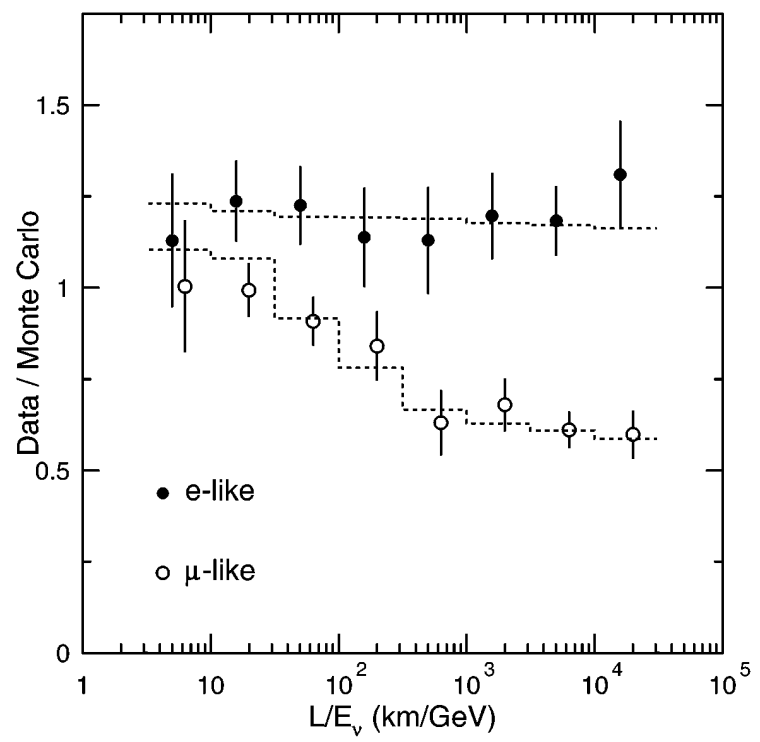
\includegraphics[width=0.5\linewidth]{superk_l_over_e.png}}%
		\subfloat[Oscillation Measurement from \cite{SuperK-Oscillations}]{
			\label{fig:superk_oscil}
			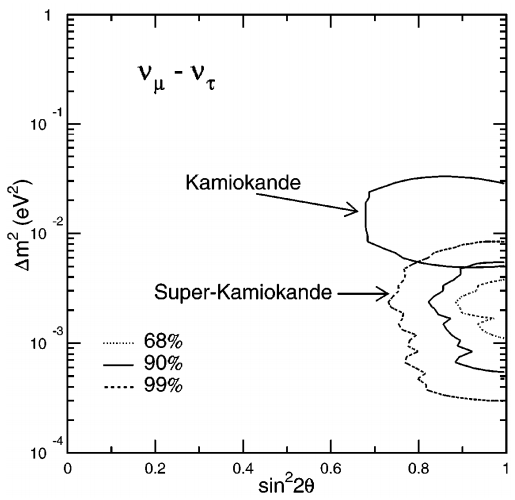
\includegraphics[width=0.5\linewidth]{superk_discovery.png}}%
	\caption{The first atmospheric neutrino oscillation measurements from the Super-K experiment. (a) The $\nu_e$-like events show no shape in L/E, as expected from a lack of neutrino oscillations. The $\nu_\mu$-like interactions, however, show a clear drop, indicating the presence of oscillation effects. (b) Using the two neutrino approximation, Super-K produced contours of the best-fit oscillation parameters for $\nu_\mu\rightarrow\nu_\tau$ oscillations. Both figures from \cite{SuperK-Oscillations}}%
\end{figure}


While investigating backgrounds, Super-Kamiokande observed an interesting deficit in the atmospheric neutrino signal.
Unlike the case in the solar neutrinos, the deficit observed by Super-K was observed solely in the muon neutrino events with no effect seem in the electron neutrinos \cite{SuperK-Oscillations}.
Using the reconstructed energy and direction of events, Super-K was able to show that the number of fully contained events of $\nu_\mu$-like interactions changed as a function of L/E - a clear signature of neutrino oscillations in the atmospheric neutrinos.
The figure, reproduced in Figure~\ref{fig:superk_l_over_e}, was used, in part, with the two flavor oscillation approximations derived in Section~\ref{subsubsec:two_flavors} to produce the first measurements, shown in Figure~\ref{fig:superk_oscil}, of the atmospheric oscillation parameters.
For the discovery of atmospheric neutrino oscillations at the same time as SNO's discovery of solar neutrino oscillations, the Super-K collaboration was jointly award the 2015 Nobel Prize \cite{NobelPrize:2015-Oscillations}.


